\documentclass[
  captions=tableheading,
  bibliography=totoc, 
  titepage=firstiscover,
]{scrartcl}

\usepackage{blindtext} %neuer input

\usepackage{longtable} % Tabellen über mehrere Seiten

\usepackage[utf8]{inputenc} %neuer input

\usepackage{scrhack}

\usepackage[aux]{rerunfilecheck} %Warnung falls nochmal kompiliert werden muss

\usepackage{fontspec} %Fonteinstellungen

\recalctypearea{}

\usepackage[main=ngerman]{babel} %deutsche Spracheinstellung

\usepackage{ragged2e} %neuer input

\usepackage{amsmath, nccmath}

\usepackage{amssymb} %viele mathe Symbole

\usepackage{mathtools} %Erweiterungen für amsmath


\DeclarePairedDelimiter{\abs}{\lvert}{\rvert}
\DeclarePairedDelimiter{\norm}{\lVert}{\rVert}

\DeclarePairedDelimiter{\bra}{\langle}{\rvert}
\DeclarePairedDelimiter{\ket}{\lvert}{\rangle}

\DeclarePairedDelimiterX{\braket}[2]{\langle}{\rangle}{
#1 \delimsize| #2
}

\NewDocumentCommand \dif {m}
{
\mathinner{\symup{d} #1}
}


\usepackage[
  math-style=ISO,
  bold-style=ISO,
  sans-style=italic,
  nabla=upright,
  partial=upright,
  warnings-off={
    mathtools-colon,
    mathtools-overbracket,
  },
]{unicode-math}

\setmathfont{Latin Modern Math}
\setmathfont{XITS Math}[range={scr, bfscr}]
\setmathfont{XITS Math}[range={cal, bfcal}, StylisticSet=1]


\usepackage[
  locale=DE,
  separate-uncertainty=true,
  per-mode=reciprocal,
  output-decimal-marker={,},
]{siunitx}

\usepackage[autostyle]{csquotes} %richtige Anführungszeichen

\usepackage{xfrac}

\usepackage{float}

\floatplacement{figure}{htbp}

\floatplacement{table}{htbp}

\usepackage[ %floats innerhalb einer section halten
  section,   %floats innerhalb er section halten
  below,     %unterhalb der Section aber auf der selben Seite ist ok
]{placeins}

\usepackage[
  labelfont=bf,
  font=small,
  width=0.9\textwidth,
]{caption}

\usepackage{subcaption} %subfigure, subtable, subref

\usepackage{graphicx}

\usepackage{grffile}

\usepackage{booktabs}

\usepackage{microtype} %Verbesserungen am Schriftbild

\usepackage[
backend=biber,
]{biblatex}

\addbibresource{../lit.bib}

\usepackage[ %Hyperlinks im Dokument
  german,
  unicode,
  pdfusetitle,
  pdfcreator={},
  pdfproducer={},
]{hyperref}

\usepackage{bookmark}

\usepackage[shortcuts]{extdash}

%\usepackage{warpcol}


\begin{document}
    \title{V101 Das Trägheitsmoment}
    \author{  
    Tobias Rücker\\
    \texorpdfstring{\href{mailto:tobias.ruecker@tu-dortmund.de}{tobias.ruecker@tu-dortmund.de}
    \and}{,} 
    Paul Störbrock\\
    \texorpdfstring{\href{mailto:paul.stoerbrock@tu-dortmund.de}{paul.stoerbrock@tu-dortmund.de}}{}
    }
    \date{Durchführung: 03.12.2019, Abgabe: 10.12.2019\vspace{-4ex}}
\maketitle
\center{\Large Versuchsgruppe: \textbf{42}}
    
    \begin{abstract}
    \centering
        \textbf{Ziel:} Messung des Trägheitsmoments verschiedener Körper und Nachweis des Satzes von Steiner
    \end{abstract}

\newpage
\tableofcontents
\newpage

% Theorie %%%%%%%%%%%%%%%%%%%%%%%%%%%%%%%%%%%%%%%%%%%%%%%%%%%%%%%%%%%%%%%%%%%%%%%%%%%%%%%%%%%%%%%%%%%%%%%%%
\section{Theorie}\justifying
\begin{align}
    \intertext{Rotationsbewegungen beschreiben Bewegungen bei denen sich eine Massenverteilung
    um eine Rotationsachse dreht. Dabei werden diese Bewegungen hauptsächlich durch die Größen
    beschrieben: dem Trägheitsmoment $I$, dem Drehmoment $M$ und der Winkelbeschleunigung $\dot{\omega}$.
    Das Trägheitsmoment beschreibt dabei eine skalare Größe, welche ein Maß der Trägheit einer Massenverteilung
    gegenüber Rotationen darstellen. Es bildet damit ein Äquivalent zur Masse in Translationsbewegungen.
    Ein Trägheitsmoment hängt dabei explizit von dem Abstand zur und der Wahl der Rotationsachse ab.
    Für eine Punktmasse zum Beispiel, lässt sich das Trägheitsmoment durch folgende Formel 
    beschreiben \cite{V101}:
    }
    I &= m  r^2 \label{eq:1}
    \intertext{Für ausgedehnte Massekörper wird diese Formel über infinitesimal kleine Massestücke aufintegriert \cite{V101}:
    }
    I &= \int r^2 \symup{d} \, m \label{eq:2}
    \intertext{Für homogene Körper lassen sich diese Integrale einfach lösen. 
    Einige Beispiele für Trägheitsmomente einfacher Körper sind das Trägheitsmoment einer homogenen Vollkugel durch seinen 
    Mittelpunkt \cite{V101}:
    }
    I_{\text{Kugel}} &= \frac{2}{5} m R^2 \label{eq:3}
    \intertext{Das Trägheitsmoment eines homogenen Vollzylinders mit der Drillachse durch den  Mittelpunkt des Bodens \cite{V101}:
    }
    I_{\text{Zylinder,v}} &= \frac{mR^2}{2} \label{eq:4}
    \intertext{Und das Trägheitsmoment eines homogenen Vollzylinders deren Drillachse senkrecht zum Mantel durch den
    Schwerpunkt verläuft \cite{V101}:
    }
    I_{\text{Zylinder,h}} &= m \left( \frac{R^2}{4}+\frac{h^2}{12} \right) \label{eq:5}
    \intertext{Bei komplexeren Körper wird versucht den Schwerpunkt durch eine Zusammensetzung einfacher Körper zu beschreiben.
    Verläuft die Drillachse parallel zu einer Achse durch den Schwerpunkt, wird das Trägheitsmoment
    mithilfe des Steinerschen Satzes berechnet \cite{V101}:
    \newline
    }
    I &= I_s+m \cdot a^2 \label{eq:6}
    \intertext{$I_s$ beschreibt dabei das Trägheitsmoment bezüglich der parallelen Drillachse durch den Schwerpunkt.
    Die skalare Größe $a$ stellt dabei den Abstand der beiden parallelen Achsen dar.
    Das Drehmoment ist definiert als die Kraft, welche an einen drehenden Körper ansetzt.
    Beschreiben lässt sich dieser durch \cite{V101}:
    \newline
    }
    \vec{M} &= \vec{F} \times \vec{r} \label{eq:7}
    \intertext{Liegt nun ein oszillierendes System vor, welches um einen Winkel $\varphi$
    ausgelenkt wird, so wirkt der Feder eine rücktreibende Kraft der Bewegung entgegen.
    Die Periodendauer der Schwingung kann dabei beschrieben werden durch \cite{V101}:
    }
    T &= 2 \pi \sqrt{\frac{I}{D}} \label{eq:8}
    \intertext{Wobei das Dremoment $M$ und die Winkelrichtgröße $D$ in folgender Beziehung
    stehen \cite{V101}:
    }
    M &= D \cdot \varphi \label{eq:9}
\end{align}

% Fehlerrechnung %%%%%%%%%%%%%%%%%%%%%%%%%%%%%%%%%%%%%%%%%%%%%%%%%%%%%%%%%%%%%%%%%%%%%%%%%%%%%%%%%%%%%%%%%%%%%%%%%%%
\section{Fehlerrechnung}\justifying
Für die Auswertung werden im folgenden diese Formeln zur Bestimmung der Fehler verwendet:
\begin{subequations}
\begin{align}
\intertext{Der Mittelwert wird berechnet mit:
}
    \overline{x} &= \frac{1}{N}\sum_{i=1}^{N} x_i \label{eq:10a}.
\intertext{Der Fehler des Mittelwerts wird berechnet:
}
    \Delta\overline{x} &= \frac{1}{\sqrt{N}} \sqrt{\frac{1}{1-N} \sum_{i=1}^{N} (x_i - \overline{x})^2} \label{eq:10b},
\intertext{Und die Gaußsche Fehlerfortpflanzung wird mit der folgenden Formel berechnet:
}
    \Delta f &= \sqrt{\sum_{i=1}^{N} \left( \frac{\delta f}{\delta x_i} \right)^2 \cdot (\Delta x_i)^2} \label{eq:10c}
\intertext{Zur Berechnung von Ausgleichsgeraden werden dabei
}
    y &= m \cdot x + b \label{eq:10d} \\ 
    m &= \frac{\overline{xy} - \overline{x} \cdot \overline{y}}{\overline{x^2} - {\overline{x}}^2} \label{eq:10e}\\
    b &= \frac{\overline{y} \cdot \overline{x^2} - \overline{xy} \cdot \overline{x}}{\overline{x^2} - {\overline{x}}^2} \label{eq:10f}
\end{align}
\end{subequations}


% Versuchsaufbau %%%%%%%%%%%%%%%%%%%%%%%%%%%%%%%%%%%%%%%%%%%%%%%%%%%%%%%%%%%%%%%%%%%%%%%%%%%%%%%%%%%%%%%%%%%%%%%%%%%%%%%%%%%%%%%%%%%%%%%%%%%%%%%%%%%%%%%%%%%
\section{Versuchsaufbau}\justifying

Benötigt werden: \textit{Eine Drillachse die durch eine Spiralfeder mit einem festen Rahmen verbunden ist, eine Stabachse der Länge $\SI{62}{\centi\meter}$, 
zwei identische zylindrische Gewichte ($\SI{261.5}{\gram}$), eine Kugel mit Aufsatz (m=$\SI{1168.5}{\gram}$, r=$\SI{7.3}{\centi\meter}$), einen Zylinder mit 
Aufsatz (m=$\SI{1525.5}{\gram}$, h=$\SI{13,95}{\centi\meter}$, d=$\SI{8}{\centi\meter}$), eine Holzpuppe mit Aufsatz ($\rho=\SI{780}{\kilo\gram\per\cubic\meter}$), 
ein Newtonmeter (von $\SI{0.1}{\newton}$ bis $\SI{1}{\newton}$), eine Drehwinkel-Messscheibe, ein Ma\ss band, eine Schieblehre, eine Stopuhr.}\\
Zu Beginn wird die Stabachse horizontal auf der Drillachse befestigt. An beiden Enden der Stabachse werden die beiden zylindrischen Gewichte angebracht.
Anschließend wird die Kugel auf die Drillachse gesteckt.
Der Zylinder wird längs auf der Drillachse aufgesteckt. 
Zum Schluss wird die Puppe in einer stehenden Position, einmal mit angelegten Armen und einmal mit ausgestreckten, senkrecht zum Körper befindlichen
Armen, auf der Drillachse befestigt.

% Versuchsdurchführung %%%%%%%%%%%%%%%%%%%%%%%%%%%%%%%%%%%%%%%%%%%%%%%%%%%%%%%%%%%%%%%%%%%%%%%%%%%%%%%%%%%%%%%%%%%%%%%%%%%%%%%%%%%%%%%%%%%%%%%%%%%%%%%%%%%%%%%%%%%
\section{Versuchsdurchführung}\justifying

Um die Trägheitsmomente der einzelnen Körper zu berechnen, soll zuerst das Trägheitsmoment der Drillachse bestimmt werden. Infolgedessen wird die
Stabachse auf der Drillachse befestigt. Die beiden zylindrischen Gewichte werden mit einem Abstand von $\SI{25}{\centi\meter}$ zur Mitte an beiden 
Enden der Stabachse angebracht. Daraufhin wird die Stabachse um einen konstanten Winkel $\varphi = \SI{20}{\degree}$ ausgelenkt und die Periodendauer mithilfe
einer Stoppuhr über drei Perioden genau zweimal gemessen. Dies wird für jede Reduzierung des Abstandes um $\SI{2.5}{\centi\meter}$ wiederholt, bis beide 
Massen bei einem Abstand von $\SI{2.5}{\centi\meter}$ zur Mitte angekommen sind.\\
Neben dem Trägheitsmoment der Drillachse ist die Federkonstante der Spiralfeder für die folgenden Trägheitsmomente wichtig. Um diese zu bestimmen 
werden die Massen von der Stabachse genommen und diese um einen Winkel von $\SI{90}{\degree}$  ausgelenkt. Nun wird das Newtonmeter an einem konstanten Abstand von 
$\SI{30}{\centi\meter}$ zur Mitte angesetzt und die Kraft der Spiralfeder übers Newtonmeter aufgenommen. Dabei wird das Newtonmeter
senkrecht zum Radius der Kreisbahn gehalten. Anschließend werden die Kräfte für eine schrittweise Erhöhung des Auslenkwinkels um $\SI{10}{\degree}$ gemessen,
bis der ein Wert von $\SI{260}{\degree}$ erreicht wird.\\
Nachdem Federkonstante und Trägheitsmoment der Drillachse bestimmt wurden, können die Trägheitsmomente des Zylinders, der Kugel und der Puppe
errechnet werden. Für die Kugel werden fünf Werte für die Schwingdauer einer Periode $T$ bei einem konstanten Winkel von $\SI{20}{\degree}$ erfasst.
Für den Zylinder werden ebenfalls fünf Messwerte für eine Periode aufgenommen, bei einem konstanten Winkel von $\SI{10}{\degree}$. 
Zuletzt werden die Schwingperioden der Puppe in Position 1 (Arme angelegt) und Position 2 (Arme ausgestreckt) gemessen. Dafür wurde der Auslenkwinkel
bei $\SI{10}{\degree}$ konstant gehalten. Um bei einer kurzen Schwingdauer verlässliche Messwerte zu erhalten, wurde die Zeitlupenfunktion einer 
Handykamera verwendet. Das Video zeigt die Schwingung der Puppe und die Stopuhr, welche den zeitlichen Verlauf der Schwingung verdeutlicht.\\
\newpage
% Auswertung %%%%%%%%%%%%%%%%%%%%%%%%%%%%%%%%%%%%%%%%%%%%%%%%%%%%%%%%%%%%%%%%%%%%%%%%%%%%%%%%%%%%%%%%%%%%%%%%%%%%%%%%%%%%%%%%%%%%%%%%%%%%%%%%%%%%%%%%%%%
\section{Auswertung}\justifying
\subsection{Maße der einzelnen Körper}
\label{sec:6.1}
\flushleft
\begin{align*}
\intertext{Zylinder:}
    &\text{Durchmesser:} &\SI{8}{\centi\meter}\\
    &\text{Höhe:}  &\SI{30}{\centi\meter}\\
    &\text{Gewicht:} &\SI{1525.5}{\gram} 
\intertext{Kugel:}
    &\text{Durchmesser:} &\SI{14.6}{\centi\meter}\\
    &\text{Gewicht:} &\SI{1168.5}{\gram}
\intertext{Puppe (Kopf):}
    &\text{Durchmesser:} &\SI{3.265}{\centi\meter}\\
    &\text{Höhe:}           &\SI{4.380}{\centi\meter} \\
    &\text{Gewicht:} &\text{\input{m_Kopf.tex}} 
\intertext{Puppe (Torso):}
    &\text{Durchmesser:} &\SI{3.89}{\centi\meter}\\
    &\text{Höhe:}  &\SI{9.625}{\centi\meter}\\
    &\text{Gewicht:} &\text{\input{m_Torso.tex}} 
\intertext{Puppe (Arm):}
    &\text{Durchmesser:} &\SI{1.65}{\centi\meter}\\
    &\text{Höhe:}  &\SI{13.25}{\centi\meter}\\
    &\text{Gewicht:} &\text{\input{m_Arm.tex}}
\intertext{Puppe (Bein):}
    &\text{Durchmesser:} &\SI{2.18}{\centi\meter}\\
    &\text{Höhe:}  &\SI{14.475}{\centi\meter}\\
    &\text{Gewicht:} &\text{\input{m_Bein.tex}}
\end{align*}

% Federkonstante --------------------------------------------------------------------------------------------------------------------------

\subsection{Die Federkonstante}

\flushleft{Für\;}\justifying die Winkelrichtgröße wurde die Formel \eqref{eq:7} mit der Formel \eqref{eq:9} gleichgesetzt. Formel \eqref{eq:7} kann durch $M = \abs{\vec{F}} \cdot \abs{\vec{r}}$
dargestellt werden, da die Kraft der rücktreibenden Kraft senkrecht zum Radius steht. Wird die gewonnene Gleichung nach $D$ umgestellt, folgt:
\begin{equation}
D = \frac{F\cdot r}{\varphi}\label{eq:11}
\end{equation}

\begin{table}[H]
    \centering
    \input{table_D.tex}
    \caption{Tabelle der Messwerte für die Winkelrichtgröße $D$}
    \label{tab:2}
\end{table}

\flushleft{Die\;}\justifying Messwerte für die rücktreibende Kraft aus Tabelle \ref{tab:2} wurden auf Grund der waagerechten Haltung des Newtonmeters
um eine Eichung von $\SI{0.05}{\newton}$ in der folgenden Rechnung ergänzt.
Werden die Werte aus \ref{tab:1} in die Formel \eqref{eq:11} eingesetzt, 
lässt sich die Winkelrichtgröße der Spiralfeder dem Mittelwert \eqref{eq:10a} der einzelnen Winkelrichtgrößen berechnen
und ergibt:

\begin{equation}
\overline{D} = \text{\input{D_mean.tex}} \label{eq:12} % Federkonstante der Spiralfeder
\end{equation}

\flushleft{Um} im folgenden für verschiedene Körper mithilfe der Formel \eqref{eq:11} das Trägheitsmoment
berechnen zu können, muss bedacht werden, dass sich das Trägheitsmoment im Schwerpunkt 
aus $I_D$ und dem Trägheitsmoment des Körpers $I_K$ zusammensetzt. Dadurch ergibt sich 
für $I_K$:
\begin{align}
    I_K = \frac{T^2 \cdot D}{4 \pi^2}-ma^2-I_D\label{eq:13}
\end{align}

\subsection{Die Drillachse}\justifying % Drillachse ---------------------------------------------------------------------------------------------------------

\begin{align}
\intertext{\flushleft{Um\;}\justifying das Trägheitsmoment der Drillachse zu bestimmen wird die Formel \eqref{eq:8} nach I umgestellt und mit Formel % Trägheitsmoment I_D ---------------------------------------------------------------------------------------------------------
\eqref{eq:6} gleichgesetzt. Die resultierende Gleichung sieht aus wie folgt:
}
T^2 = I_S \cdot \frac{4\pi^2}{D} &+ \frac{m_k \cdot 4\pi^2}{D} \cdot a^2 \label{eq:14}
\intertext{Hierbei wird festgestellt, dass
}
b &= I_S \cdot \frac{4\pi^2}{D} \label{eq:15}
\intertext{entspricht.
Daraus folgt für das Trägheitsmoment der Drillachse:
\newline
}
I_D &= \frac{b \cdot D}{4 \pi^2} \label{eq:16}
\end{align}

\begin{table}[H]
    \centering
    \input{table_IStab.tex}
    \caption{Tabelle der Messwerte für das Trägheitsmoment der Stabachse $I_D$}
    \label{tab:1}
\end{table}

\flushleft{Für} die Berechnung wurde für einen Abstand die Periodendauer zweimal gemessen (Wert1, Wert2) und in der Tabelle \ref{tab:1}
zusammengetragen. Diese zwei Werte wurden gemittelt und auf eine Periode normiert.

\flushleft{Mithilfe\;}\justifying des Pyton Befehls linregress() \cite{numpy} lässt sich die Geradengleichung
des folgenden Graphen \ref{fig:1} bestimmen. 
\flushleft{Dabei\;}\justifying sehen die Steigung $m$ und der Schnittpunkt der y-Achse $b$ des Graphen \ref{fig:1} folgendermaßen aus:

\begin{subequations}
\begin{align}
m &= \text{\input{slope.tex}}\label{eq:17a}\\
b &= \text{\input{intercept.tex}}\label{eq:17b}
\end{align}
\end{subequations}

\begin{figure}[H]
    \centering
    \includegraphics[width=0.75\textwidth]{plot.pdf}
    \caption{Lineare Regression für $I_{Stab}$}
    \label{fig:1}
\end{figure}

\flushleft{Aus\;}\justifying der linearen Regression lässt sich das Trägheitsmoment der Drillachse mit Formel \eqref{eq:16} bestimmten:
\begin{equation}
I_D = \input{I_D.tex}\label{eq:18} % Trägheitsmoment Drillachse
\end{equation}

\subsection{Der Zylinder}\justifying % Zylinder ---------------------------------------------------------------------------------------------------------
\label{sec:5.5}
\begin{table}[H]
    \centering
    \input{table_I.tex}
    \caption{Tabelle der Messwerte für die Perioden $T$ der einzelnen Körper}
    \label{tab:3}
\end{table}

\begin{subequations}
\begin{align}
\intertext{\flushleft{Die\;}\justifying Werte für die Periodendauer aus der Tabelle \ref{tab:3} wurden für alle folgenden Berechnungen auf eine Nachkommastelle gerundet.
Für den experimentellen Wert des Trägheitsmoments des Zylinders wurde die Formel \eqref{eq:14} nach $I_S$ umgestellt. Die resultierenden $I_S$'s wurden
anschließend gemittelt. Daraus folgt das experimentelle Trägheitsmoment des Zylinders mit den Werten aus Tabelle \ref{tab:3}, der Formel \eqref{eq:10a} 
und einer Masse von $\SI{1525.5}{\gram}$:
\newline
}
\overline{I_{Zy, exp.}} &= \input{I_Zylinder_mean.tex}\label{eq:19a}
\intertext{\flushleft{Das\;}\justifying theoretische Trägheitsmoment des Zylinders wurde mit der Formel \eqref{eq:5} und den Werten für $T$ aus Tabelle 
\ref{tab:3} bestimmt und lautet:
\newline
}
I_{Zy, lit.} &= \input{I_Zylinder_Theorie.tex}\label{eq:19b}
\intertext{\flushleft{Der\;}\justifying daraus resultierende relative Fehler des Trägheitsmoments vom Zylinder beträgt:
\newline
}
\frac{\overline{I_{Zy, exp.}} - I_{Zy, lit.}}{I_{Zy, lit.}} &= \input{RF_I_Zylinder.tex}\label{eq:19c}
\end{align}
\end{subequations}

\subsection{Die Kugel}\justifying % Kugel ---------------------------------------------------------------------------------------------------------

\flushleft{Das\;}\justifying experimentelle Trägheitsmoment der Kugel wurde mit der selben Formel \eqref{eq:14} bestimmt, wie das des Zylinders.
Die Werte für $T$ werden der Tabelle \ref{tab:3} entnommen und ebenfalls auf eine Nachkommastelle gerundet. 
Demnach lautet der experimentelle Wert des Trägheitsmoments analog zu Abschnitt \ref{sec:5.5}:
\begin{subequations}
\begin{align}
\overline{I_{Ku, exp.}} &= \input{I_Kugel_mean.tex} \label{eq:20a}
\intertext{\flushleft{Das\;}\justifying theoretische Trägheitsmoment der Kugel wurde mit der Formel \eqref{eq:3} und den Werten 
aus Tabelle \ref{tab:3} bestimmt:
}
I_{Ku, lit.} &= \input{I_Kugel_Theorie.tex} \label{eq:20b}
\intertext{\flushleft{Der\;}\justifying relative Fehler des Trägheitsmoments der Kugel ist:
}
\frac{\overline{I_{Ku, exp.}} - I_{Ku, lit.}}{I_{Ku, lit.}} &= \input{RF_I_Kugel.tex} \label{eq:20c}
\end{align}
\end{subequations}

\subsection{Die Puppe}\justifying % Puppe ---------------------------------------------------------------------------------------------------------

\flushleft{Die\;}\justifying folgenden zwei Bilder \ref{fig:2} approximieren die Gliedmaßen der Puppe als Zylinder für die folgenden 
Berechnungen. Bild \subref{fig:2a} stellt die Puppe in Position 1 mit angezogenen Armen und Bild \subref{fig:2b} in Position 2 mit 
ausgestreckten Armen dar.

\begin{figure}[H]
\caption{Positionen der Puppe}
\label{fig:2}
    \begin{subfigure}{0.495\linewidth}
        \centering
        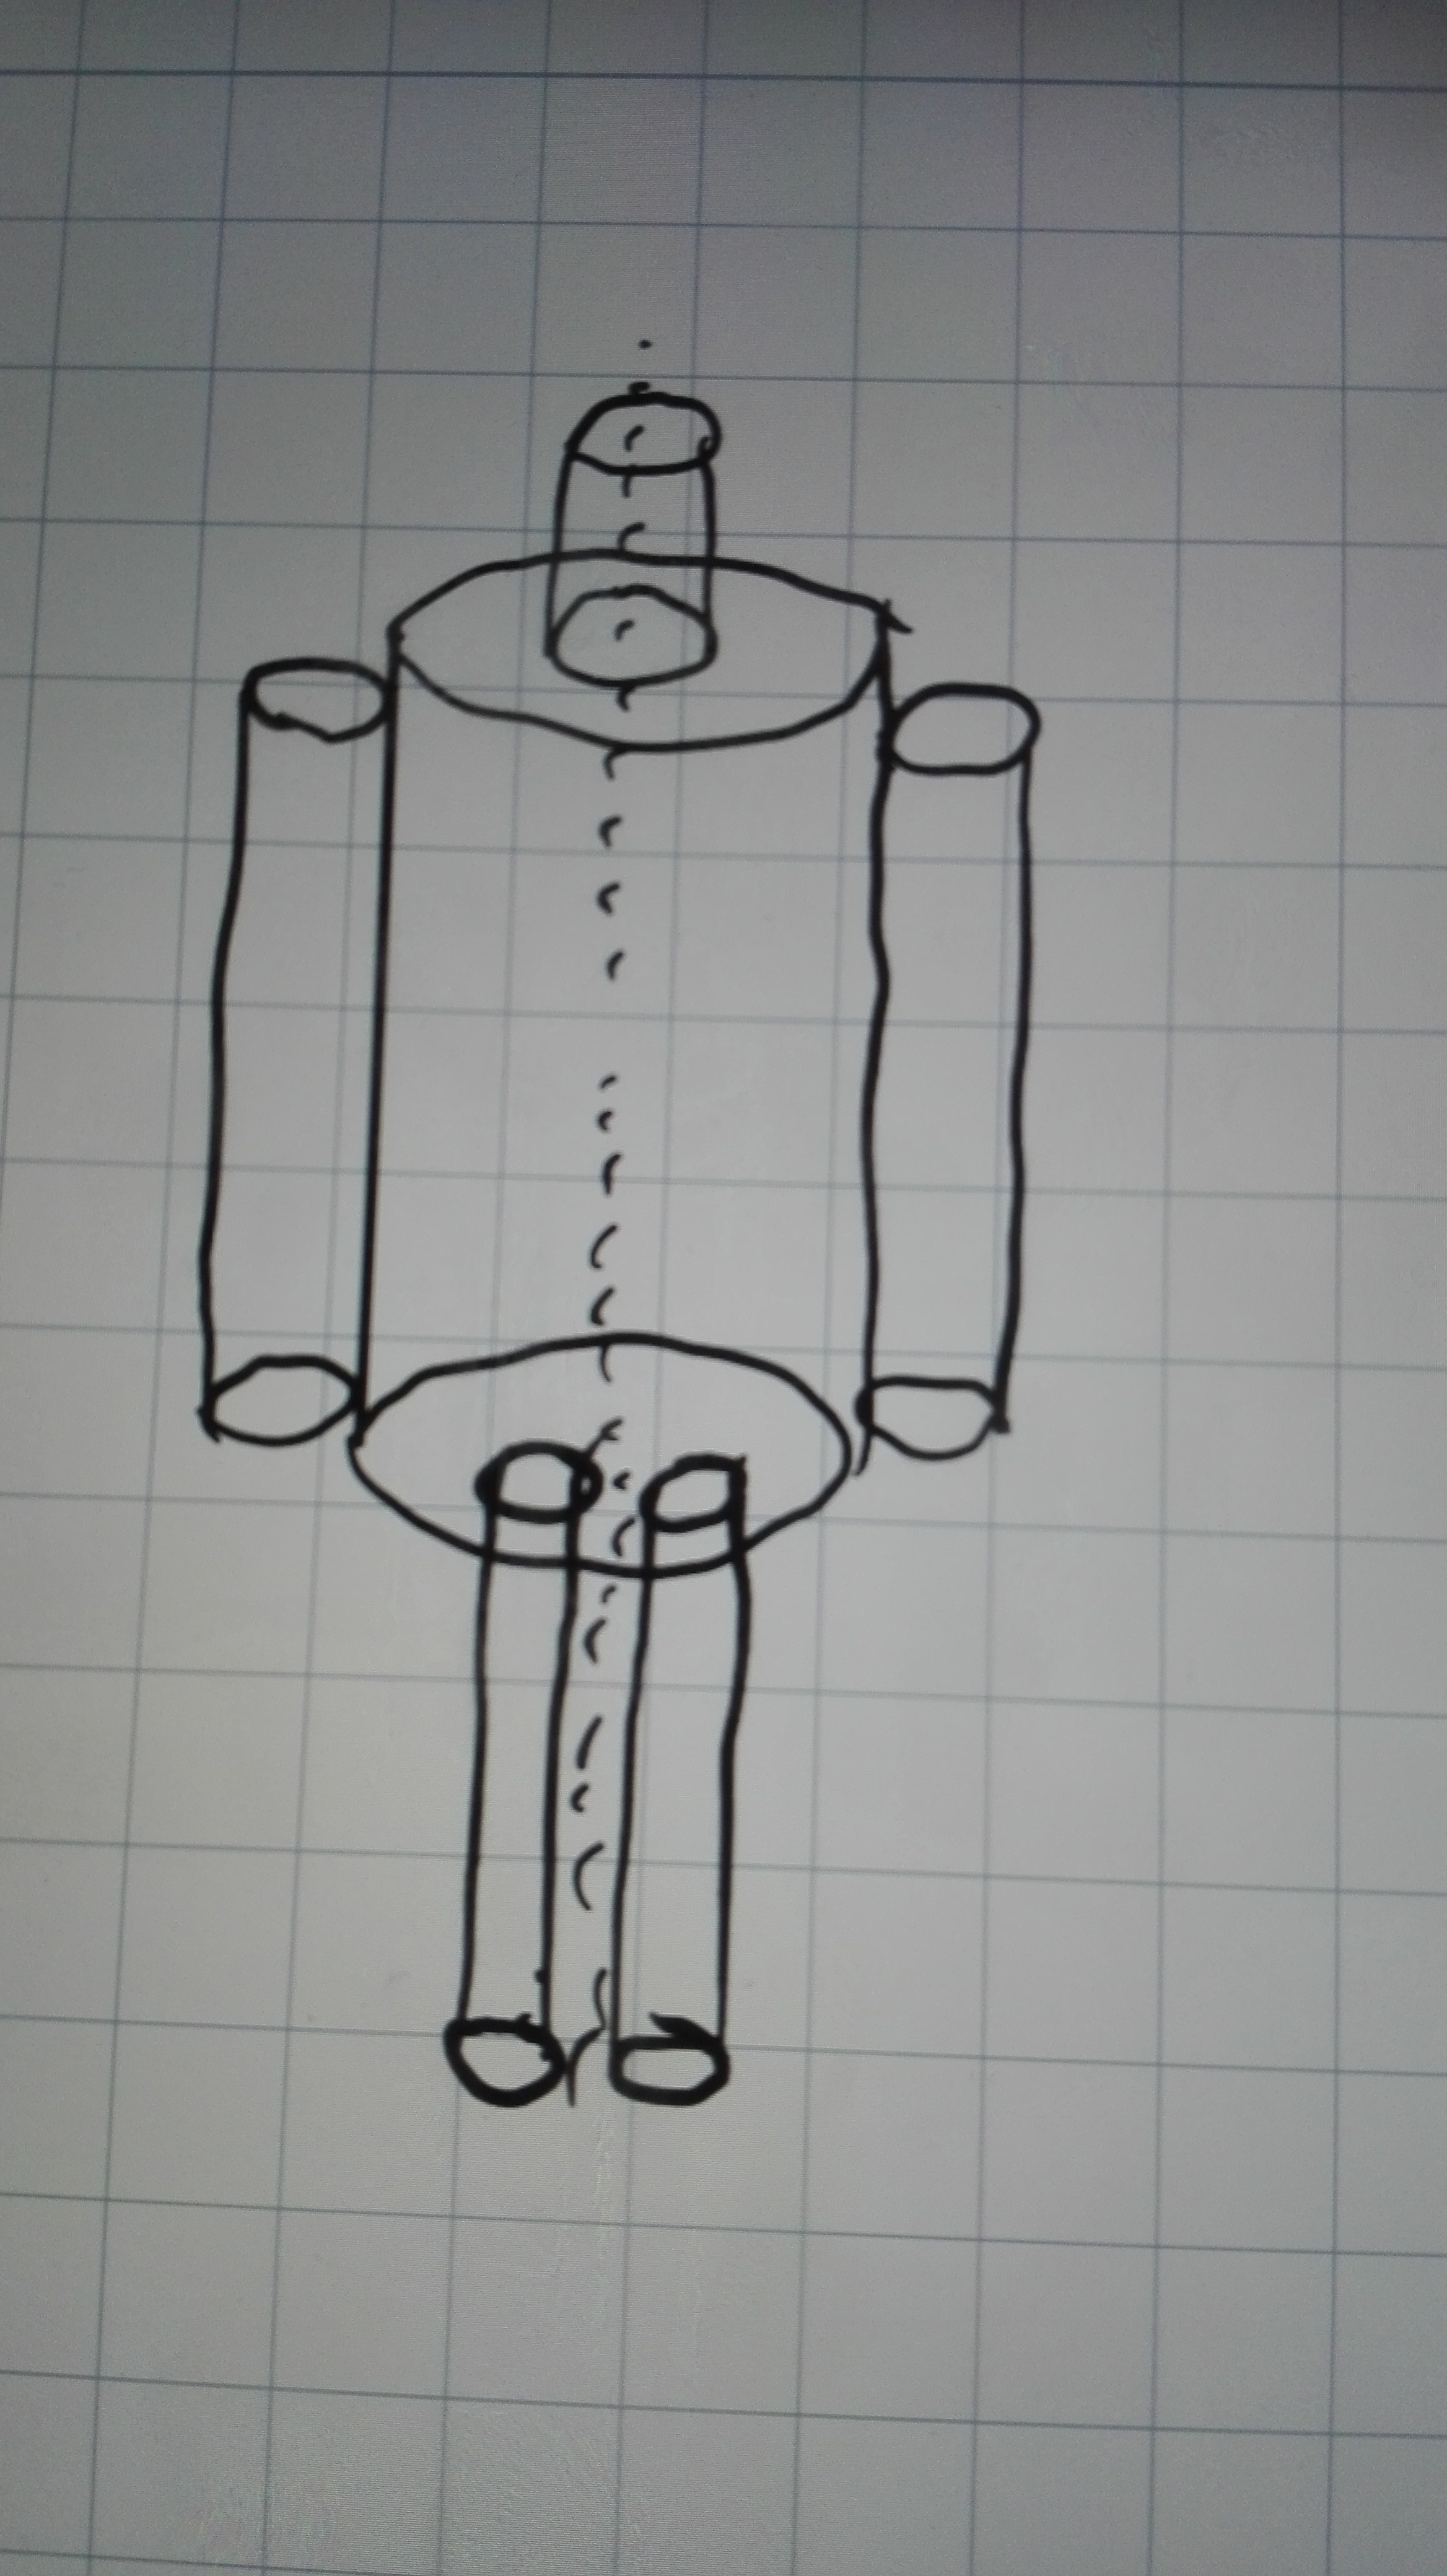
\includegraphics[width=\textwidth]{images/puppe_an.jpg}
        \caption{Puppe mit angezogenen Armen (Pos. 1)}
        \label{fig:2a}
    \end{subfigure}
    \begin{subfigure}{0.495\linewidth}
        \centering
        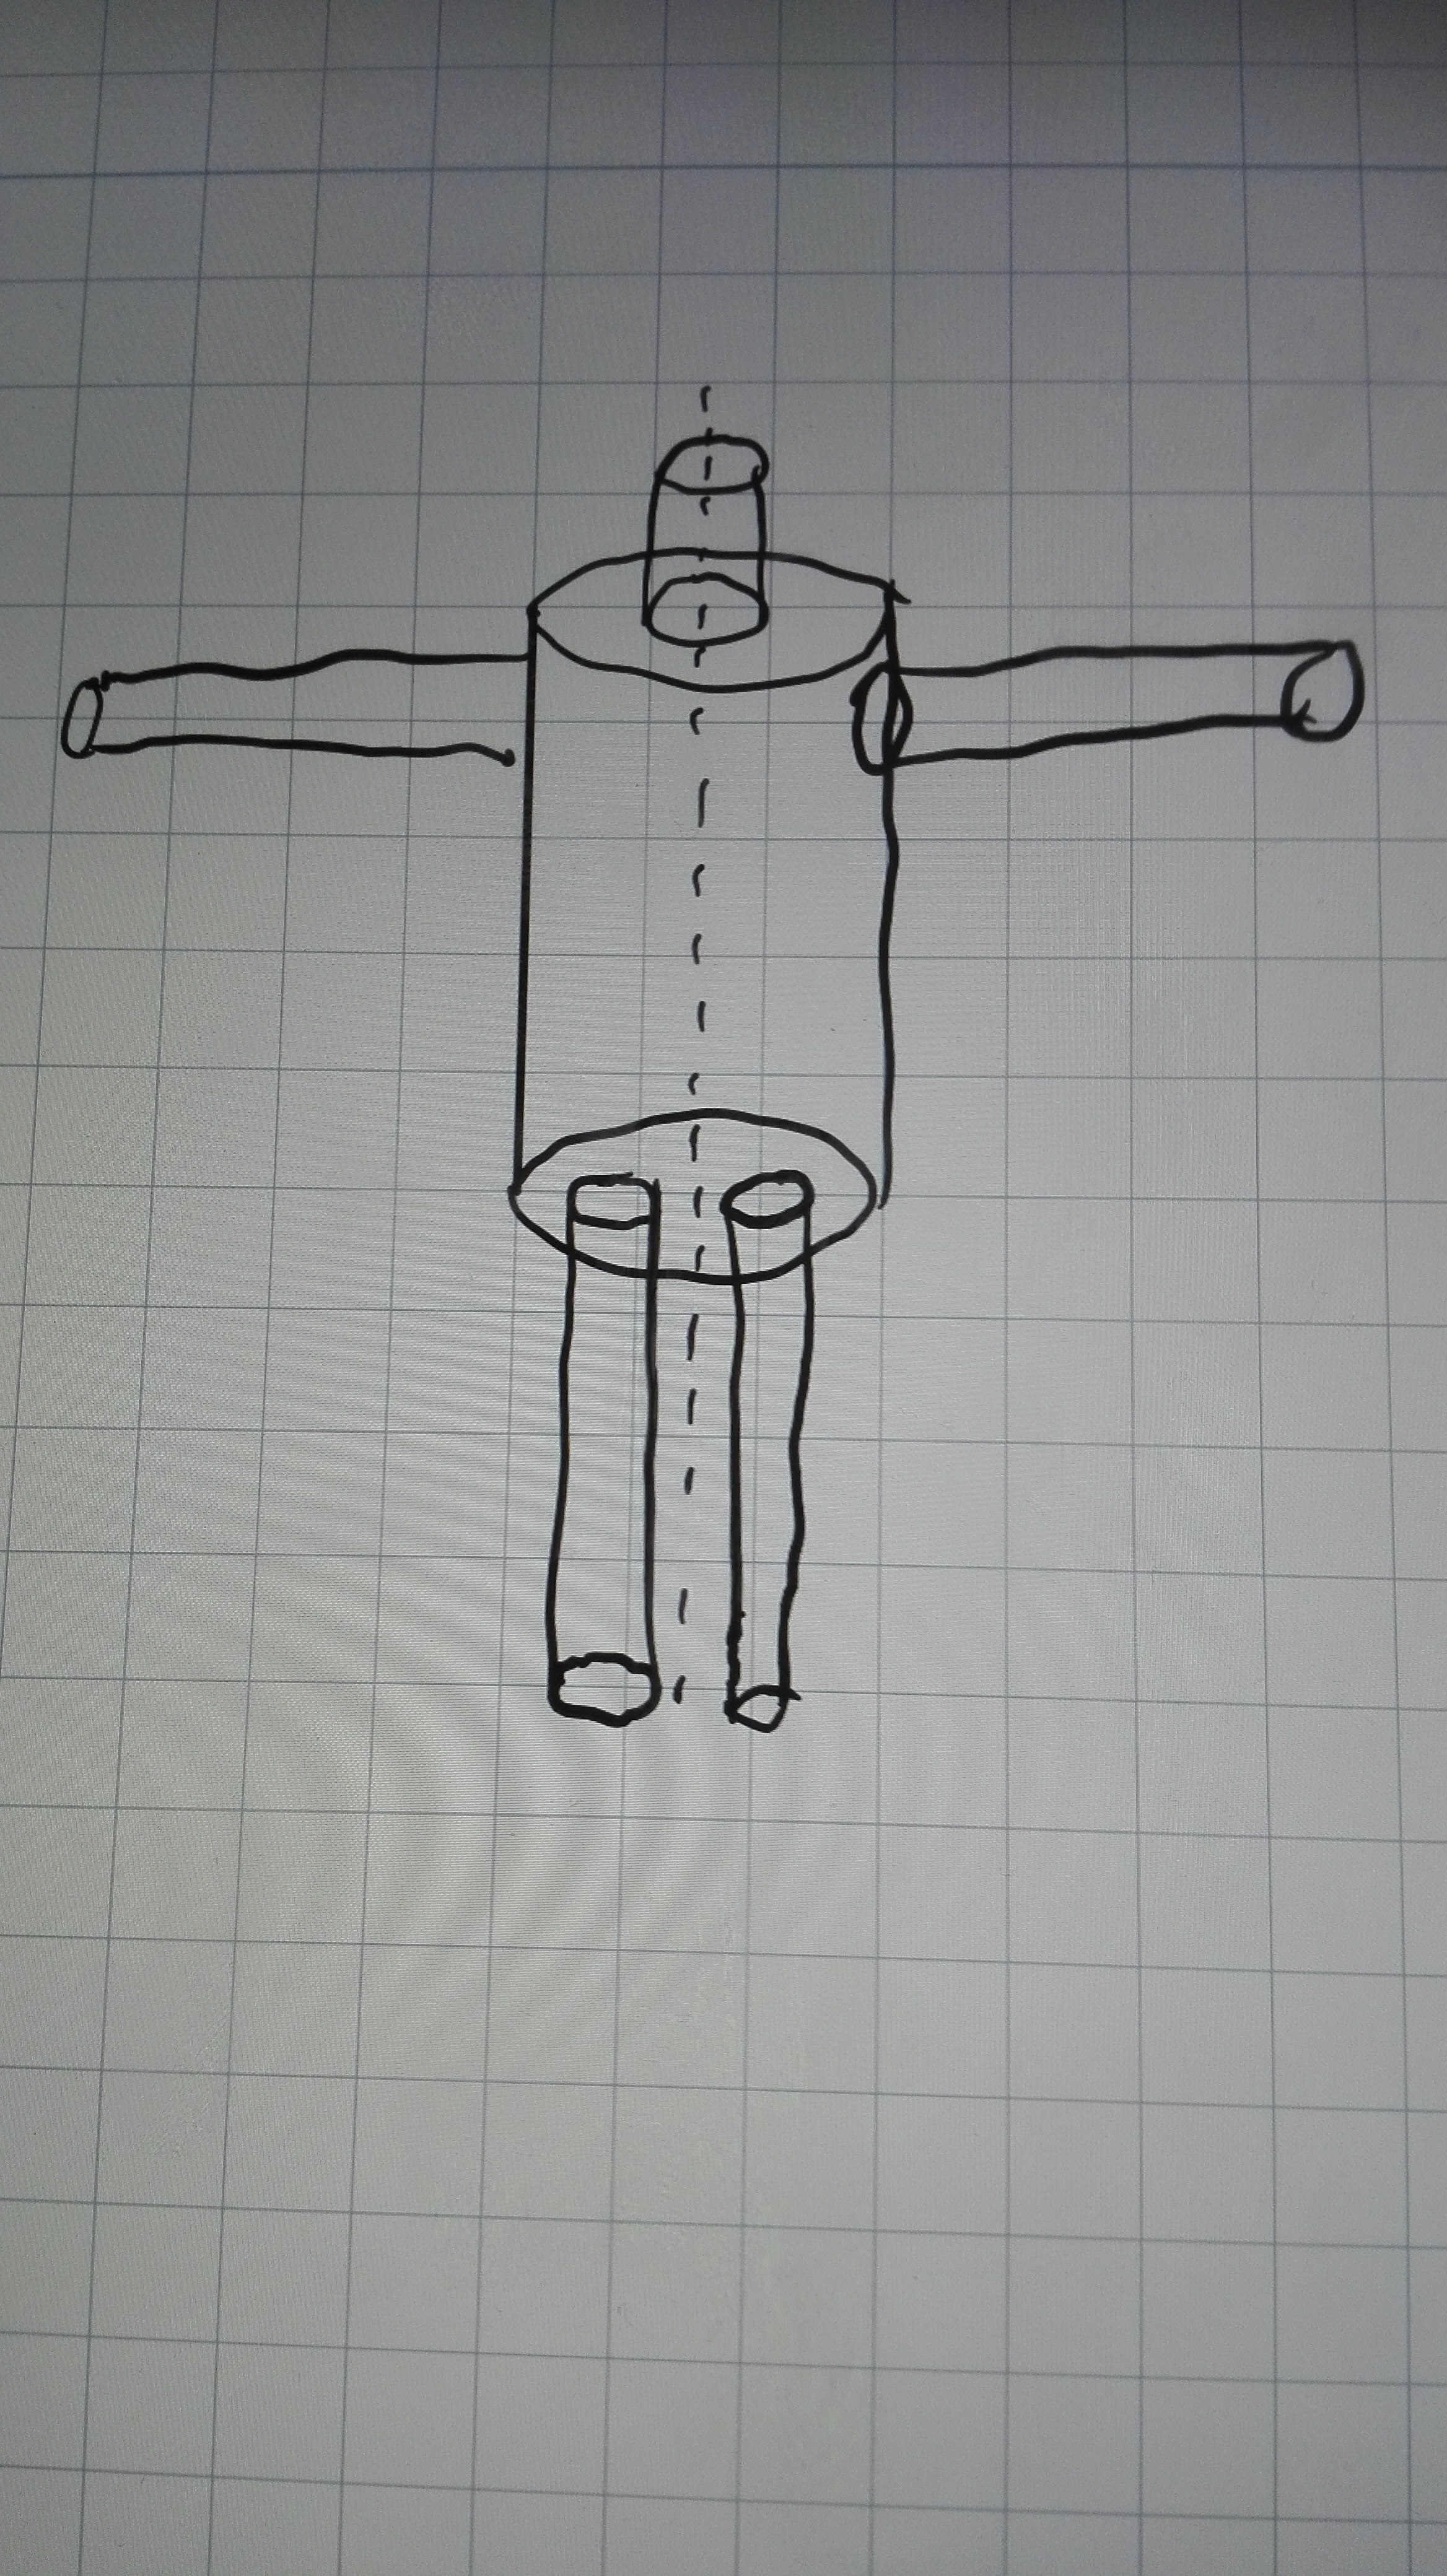
\includegraphics[width=\textwidth]{images/puppe_aus.jpg}
        \caption{Puppe mit ausgestreckten Armen (Pos. 2)}
        \label{fig:2b}
    \end{subfigure}
\end{figure}
\flushleft{Die\;}\justifying Massen der einzelnen Zylinder wurden mithilfer der Formel $m= \rho \cdot V$ bestimmt und lauten wie folgt:

\begin{subequations}
\begin{align}
\text{Kopf: \input{m_Kopf.tex}}\label{eq:21a}\\
\text{Torso: \input{m_Torso.tex}}\label{eq:21b}\\
\text{Arm: \input{m_Arm.tex}}\label{eq:21c}\\
\text{Bein: \input{m_Bein.tex}}\label{eq:21d}
\end{align}
\end{subequations}

\flushleft{$V$\;}\justifying stellt dabei die verschiedenen Zylindervolumen dar

\begin{subequations}
\begin{align}
 V_{\text{Kopf}} &= \input{V_Kopf.tex}\label{eq:22a}\\
 V_{\text{Torso}} &= \input{V_Torso.tex}\label{eq:22b}\\
 V_{\text{Arm1,2}} &= \input{V_Arm.tex}\label{eq:22c}\\
 V_{\text{Bein1,2}} &= \input{V_Bein.tex}\label{eq:22d},
\end{align}
\end{subequations}

\flushleft{während\;}\justifying $\rho$ die Dichte von Buchenholz darstellt \cite{Holzdichte}:
\begin{align}
    \rho = \SI{760}{\kilo\gram\meter\tothe{-3}}\label{eq:23}.
\end{align}

\subsubsection{Puppe in Position 1}\label{sec:Puppe1} % Puppe 1 ---------------------------------------------------------------------------------------------------------

\flushleft{Um\;}\justifying das experimentelle Trägheitsmoment der Puppe in Position 1 berechnen zu können, werden die die Trägheitsmomente der
einzelnen Zylinder mit der Formel \eqref{eq:13} und den Werten aus Tabelle \ref{tab:3} bestimmt. Die individuellen Trägheitsmomente werden
aufsummiert um das Trägheitsmoment der Puppe für die einzelnen Periodendauern zu erhalten. Abschließend werden die Trägheitsmomente
mit der Mittelwertsformel \eqref{eq:10a} gemittelt um auf das Gesamtträgheitsmoment zu kommen: 
\begin{subequations}
\begin{align}
\intertext{Demnach folgt aus der Summe der einzelnen $I_K$'s}
I_{P1,sum.} &= \sum_{i=1}^{6} I_{P1} \qquad \text{mit\;} I_K = I_{P1,2}\label{eq:24a}
\intertext{und dem gebildeten Mittel der $I_{K,sum.}$'s das experimentelle Trägheitsmoment der Puppe in Position 1:
}
\overline{I_{P1,exp.}} &= \input{I_Puppe_an_exp_mean.tex}\label{eq:24b}
\intertext{Bei dem theoretischen Trägheitsmoment der Puppe in Position 1 wird ähnlich verfahren. Die Trägheitsmomente der einzelnen Zylinder werden 
mit der Formel \eqref{eq:4} bestimmt und aufsummiert. Daraus folgt der theoretische Wert:
}
I_{P1,lit.} &= \input{I_Puppe_an_theo.tex}\label{eq:24c}
\intertext{Der relative Fehler des Trägheitsmoments der Puppe in Position 1 ist:
}
\frac{\overline{I_{P1, exp.}} - I_{P1, lit.}}{I_{P1, lit.}} &= \input{RF_I_Puppe_an.tex}\label{eq:24d}
\end{align}
\end{subequations}

\subsubsection{Puppe in Position 2}\justifying \label{sec:Puppe2} % Puppe 2 ---------------------------------------------------------------------------------------------------------

\flushleft{Für\;}\justifying das Gesamtträgheitsmoment der Puppe in Position 2 wird identisch verfahren wie für das Trägheitsmoment der 
Puppe in Position 1. Der einzige Unterschied liegt in der Periodendauer aus Tabelle \ref{tab:3}. Werden die einzelnen Trägheitsmomente
aufsummiert und der Mittelwert \eqref{eq:10a} berechnet wie in Abschnitt \ref{sec:Puppe1} beschreiben, folgt:
\begin{subequations}
\begin{align}
\overline{I_{P2,exp.}} &= \text{\input{I_Puppe_aus_exp_mean.tex}}\label{eq:25a}
\intertext{Das theoretische Trägheitsmoment der Puppe in Position 2 wird wieder mit Formel \eqref{eq:4} bestimmt:
}
I_{P2,lit.} &= \input{I_Puppe_aus_theo.tex}\label{eq:25b}
\intertext{Demnach folgt ein relativer Fehler des Trägheitsmoments der Puppe in Position 2 von:
}
\frac{\overline{I_{P2, exp.}} - I_{P2, lit.}}{I_{P2, lit.}} &= \input{RF_I_Puppe_aus.tex}\label{eq:25c}
\end{align}
\end{subequations}
\newpage

% Diskussion %%%%%%%%%%%%%%%%%%%%%%%%%%%%%%%%%%%%%%%%%%%%%%%%%%%%%%%%%%%%%%%%%%%%%%%%%%%%%%%%%%%%%%%%%%%%%%%%%%%%%%%%%%%%%%%%%%%%%%%%%%%%%%%%%%%%%%%%%%%

\section{Diskussion}\justifying
Nach der Auswertung folgt nun eine kurze Diskussion der berechneten Werte.\\
Die Winkelrichtgröße D \eqref{eq:12} scheint in einer passenden
Größenordnung vorzuliegen, allerdings lässt sich anhand der Formel \eqref{eq:11}
und der Tabelle \ref{tab:2} ein Fehler in der Messung erkennen.
Da die Winkelrichtgröße grundsätzlich konstant sein sollte, ergibt sich bei einem
doppelt so großen Winkel eine doppelt so große Kraft. Dies ist hier nicht direkt der Fall
wie die Werte für \SI{90}{\degree} und \SI{180}{\degree} zeigen. Diese Messungenauigkeit
ergibt sich aus dem Problem des Nullpunkts beim Newtonmeter. In der Messung wurde das
Newtonmeter senkrecht an die ausgelenkte Stange gehalten, um die Federkraft zu ermitteln. Dabei kann es
beim Loslassen der Stange passieren, dass die Feder des empfindlichen Newtonmeters bereits ausgelenkt wurde oder 
erst nach kurzer Zeit ausgelenkt wurde, sodass sich eine kleine Abweichung in der Messung ergibt.
Dabei musste für die Werte berücksichtigt werden, dass das Newtonmeter auf Messungen im 
Schwerefeld der Erde geeicht wurde und dementsprechend auf alle Werte für F in Tabelle 
\ref{tab:2} noch $\SI{0.05}{\newton} $ addiert werden muss.
Zudem ergibt sich eine gewisse Ungenauigkeit beim Einstellen des Winkels. 

\flushleft{Für\;}\justifying das Trägheitsmoment des Stabs wurde der Wert aus Formel \eqref{eq:16} bestimmt.
Bei dem Versuch wurde der Stab, auf dem sich die beiden Zylinder befanden, als masselos angenommen  und
die Zylinder als Punktmassen angenähert. Dabei wurde für die Auswertung bei der Periodendauer
nur die erste Nachkommastelle verwendet, da aufgrund der menschlichen Reaktionszeit sich
automatisch eine Ungenauigkeit für niedrigere Nachkommastellen ergibt.
Der Wert für das Trägheitsmoment $I_D$ wirkt dabei erstmal ziemlich klein, allerdings kann
dies täuschen, da eine theoretische Berechnung aufgrund der fehlenden Masse für den 
Drillachse nicht durchgeführt werden konnte. Allerdings führen die Annäherungen in der 
Regel zu einer bestimmten Ungenauigkeit.
Der Graph \ref{fig:1} mit seinen Messwerten aus Tabelle \ref{tab:1} liegt dabei ohne große 
Abweichungen vor und spiegelt die in Formel \eqref{eq:14} gegebene Relation gut wieder.

\flushleft{Durch\;}\justifying die beiden Messungenauigkeiten in $D$ und $I_D$ ergibt
sich auch automatisch ein Fehler für die Trägheitsmomente der verschiedenen Körper.

\flushleft{Werden\;}\justifying nun nur die Literaturwerte des Zylinders und der Kugel betrachtet lässt sich ein gutes Verhhältnis erkennen.
Der Literaturwert des Zylinders \eqref{eq:19b} beschreibt ein größeres Trägheitsmoment als das der Kugel \eqref{eq:20b}. Dies war zu erwarten,
da der Zylinder eine größere Masse und Breite besitzt. 

\flushleft{Die\;}\justifying experimentellen Werte, auf der anderen Seite, geben das Gegenteil der erwarteten Werte wieder. Beide Trägheitsmomente, 
das der Kugel \eqref{eq:20a} und das des Zylinders \eqref{eq:19a}, sind negativ, was pyhsikalisch nicht möglich ist. Dennoch ist das Trägheitsmoment 
des Zylinders größer, welches den Verdacht schöpft, dass das Trägheitsmoment der Drillachse \eqref{eq:18} nach Formel \eqref{eq:13} zu groß 
sein könnte. Ist dies nicht der Fall, könnte die Negativität auf einen oder mehrere systematische Fehler zurückgeführt werden. Diese würden 
in der Form von Messungenauigkeiten auftreten. Einige Beispiele für Messungenauigkeiten wären die menschliche Reaktionszeit beim Stoppen der Zeit
für die Periodendauern, die ignorierten Messfehler bei der Bestimmung der Volumina und die Bestimmung der Winkelauslenkung nach Augenmaß.
Der relative Fehler für Kugel \eqref{eq:20c} und Zylinder \eqref{eq:19c} ist in beiden Fällen signifikant. 

\flushleft{Im\;}\justifying Fall der Puppe bestehen identische Vorraussetzung wie bei der Kugel und beim Zylinder. Die Puppe weist für beide Positionen
\eqref{eq:24b} und \eqref{eq:25a} ein negatives experimentelles Trägheitsmoment auf. Die Messungenauigkeiten existieren analog zu denen der Kugel, 
bzw. des Zylinders. Jedoch könnte bei der Puppe die Approximation der einzelnen Glieder als Zylinder einen relevanten Beitrag leisten. 
Ähnlich wie bei dem Zylinder und der Kugel beschrieben die Literaturwerte \eqref{eq:24c} und \eqref{eq:25b} das erwartete Verhhältnis der beiden 
Positionen. Nämlich, dass die Puppe mit ausgestreckten Arme ein höheres Trägheitsmoment hat, als mit angezogenen Armen. 
% --------------------------------------------------------------------------------------------------------------------------------------------------

\flushleft{Für\;}\justifying den Zylinder ergibt sich ein relaiver Fehler von $37\%$, welcher  sich
durch die bereits genannten Fehler erklären ließe. 


\flushleft{Für\;}\justifying die Kugel ergibt sich ein relativer Fehler von $-34\%$, welcher wie beim Zylinder durch
die Messungenauigkeit in $D$ und $I_D$ begründet werden könnte.
Allerdings zeigt sich, dass das Trägheitsmoment der Kugel kleiner als das Trägheitsmoment
des Zylinders ist. Dies erscheint aufgrund der gemessenen und berechneten Größen in Abschnitt \ref{sec:6.1}
sinnvoll. Beim Zylinder ist Zum einen die Masse größer, zum  anderen sind die Massepunkte weiter 
von der Rotationsachse entfernt als bei der Kugel.
\newpage

\flushleft{Bei\;}\justifying der Berechnung des experimentellen Trägheitsmoment der Puppe ergibt
sich, im Gegensatz zur Kugel und dem Zylinder, bei beiden Positionen
 ein negatives Trägheitsmoment. Dies kann nicht stimmen, da das Trägheitsmoment
 nach der Definition in der Physik positiv definiert sein müsste. Dieser Fehler ließe
 sich nicht nur durch die bereis bekannten Fehler erklären. Zu diesen Fehlern kommt
 noch hinzu, dass die Körperform der Puppe bei der theoretischen Berechnung
 der Formel \eqref{eq:13} nur angenähert wurde und dementsprechend nicht
 realitätsgetreu ist. Außerdem war das genaue Material der Puppe nicht bekannt.
 Daher wurde angenommen, dass es sich bei dem Material um Buchenholz handele.
 Dadurch entsteht auch der große relative Fehler bei den Formeln \eqref{eq:24d} und \eqref{eq:25a}.
 Trotzdem lässt sich aus den experimentellen Trägheitsmomenten erkennen, dass
 sich die Puppe in Position 2 langsamer bewegt hat, als in Position 1, da das
 Trägheitsmoment in Formel \eqref{eq:24b} geringer ist als das Trägheitsmoment in
 Formel \eqref{eq:25a}.

 \flushleft{Anhand\;}\justifying der vorliegenden Fehler und angenäherten Körperformen lässt sich der Satz von Steiner nicht 
 nachweisen, da die vorgenommenen Approximationen zu teilweise negativen Trägheitsmomenten führen.

\newpage

\printbibliography
\end{document}